% -*- latex -*-
%%%%%%%%%%%%%%%%%%%%%%%%%%%%%%%%%%%%%%%%%%%%%%%%%%%%%%%%%%%%%%%%
%%%%%%%%%%%%%%%%%%%%%%%%%%%%%%%%%%%%%%%%%%%%%%%%%%%%%%%%%%%%%%%%
%%%%
%%%% This text file is part of the source of 
%%%% 'Parallel techniques'
%%%% by Ángel de Vicente, copyright 2019
%%%%
%%%% TO DO:
%%%%
%%%% mpi-collectives.tex : introduction to MPI concepts
%%%%      Slides adapted from
%%%%       https://doc.itc.rwth-aachen.de/display/VE/PPCES+2016
%%%%
%%%%%%%%%%%%%%%%%%%%%%%%%%%%%%%%%%%%%%%%%%%%%%%%%%%%%%%%%%%%%%%%
%%%%%%%%%%%%%%%%%%%%%%%%%%%%%%%%%%%%%%%%%%%%%%%%%%%%%%%%%%%%%%%%

This chapter builds on chapter \ref{ch:mpi-slides}. The concepts are just the
same, but we learn how to exchange messages not only from one process to
another, but ``collective'' messages, those involving all processes in a
communicator (in our case, always the communicator \textit{MPI\_COMM\_WORLD},
i.e. all processes).

\Level 0 {MPI collective routines}
\label{sec:collective-mpi}

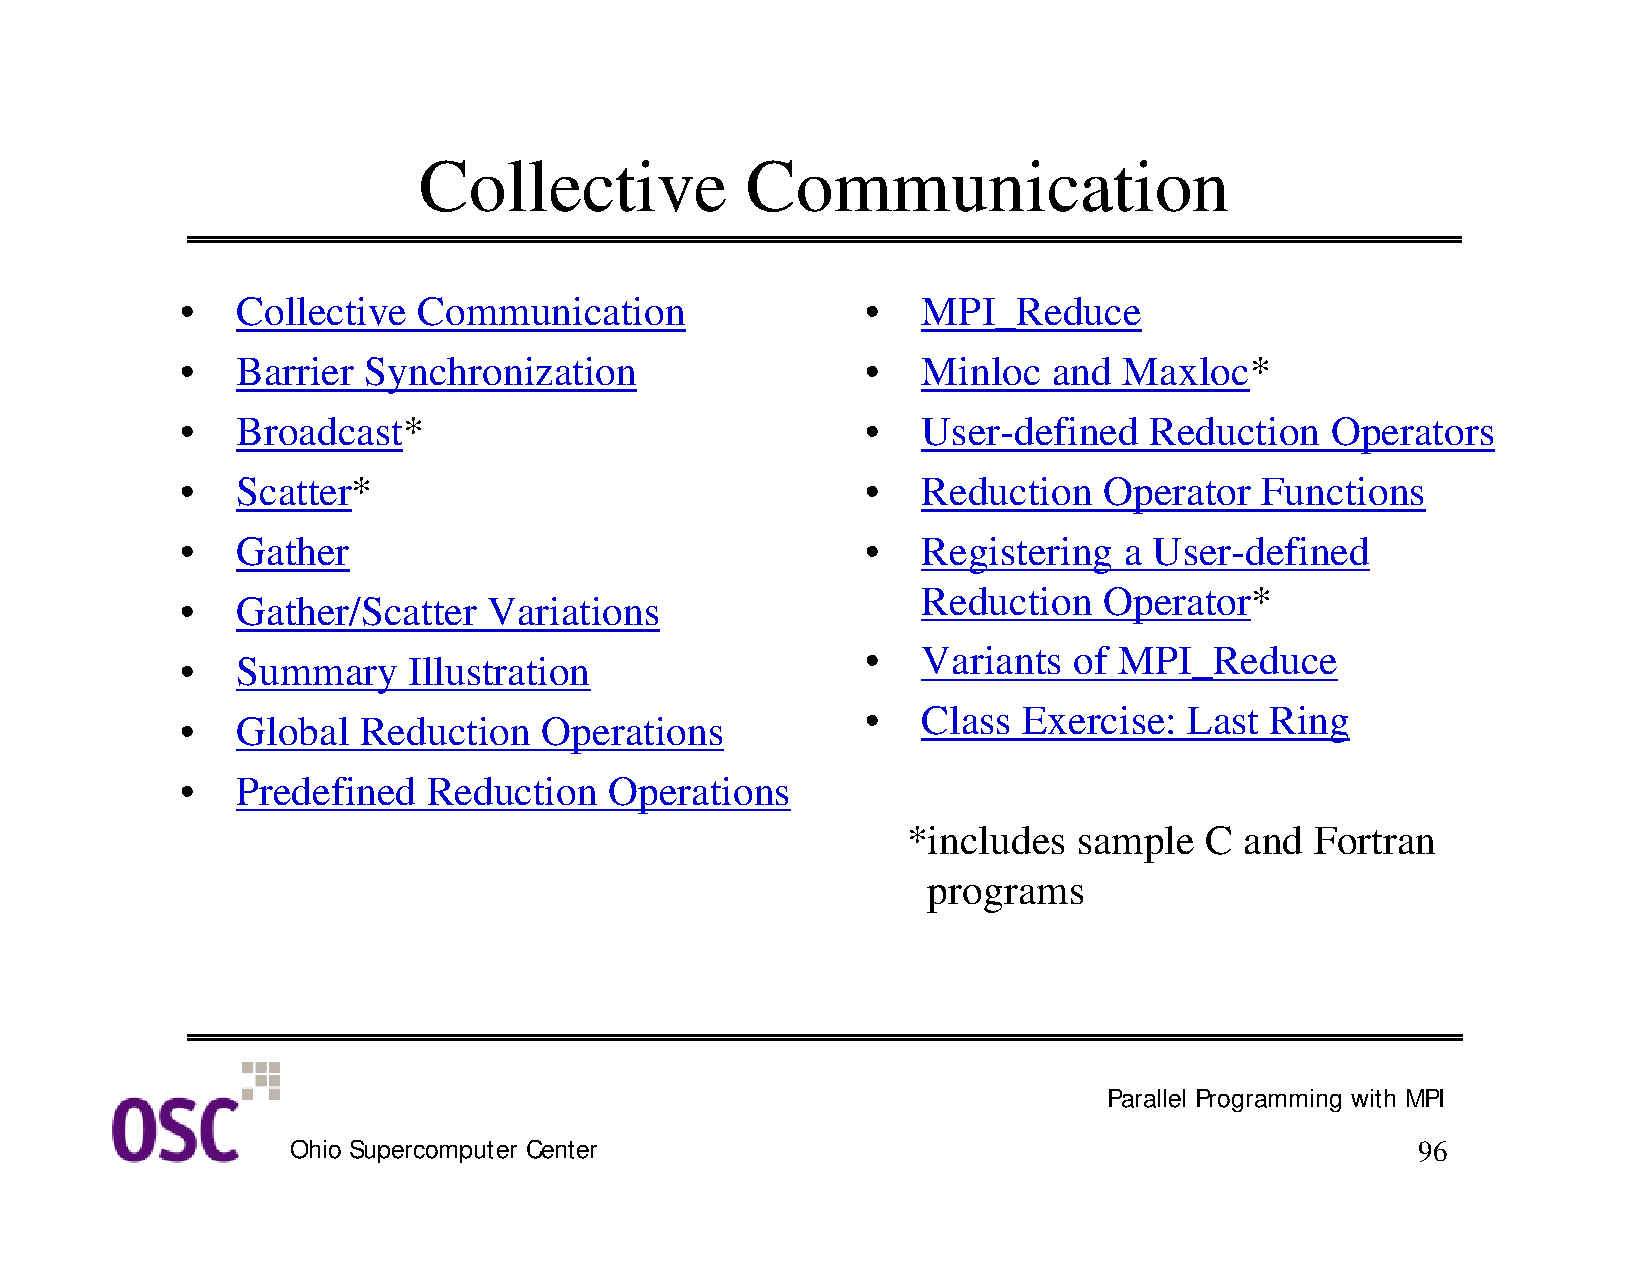
\includepdf[frame=true,scale=0.98,landscape,pages=-]{graphics/mpi_part2.pdf}}

MPI has MANY other routines. You can check all of them, together with their
syntax and some usage examples at the OpenMPI webpage
\url{https://www.open-mpi.org/doc/v4.0/}

\begin{figure}[!htbp]
  \centering
  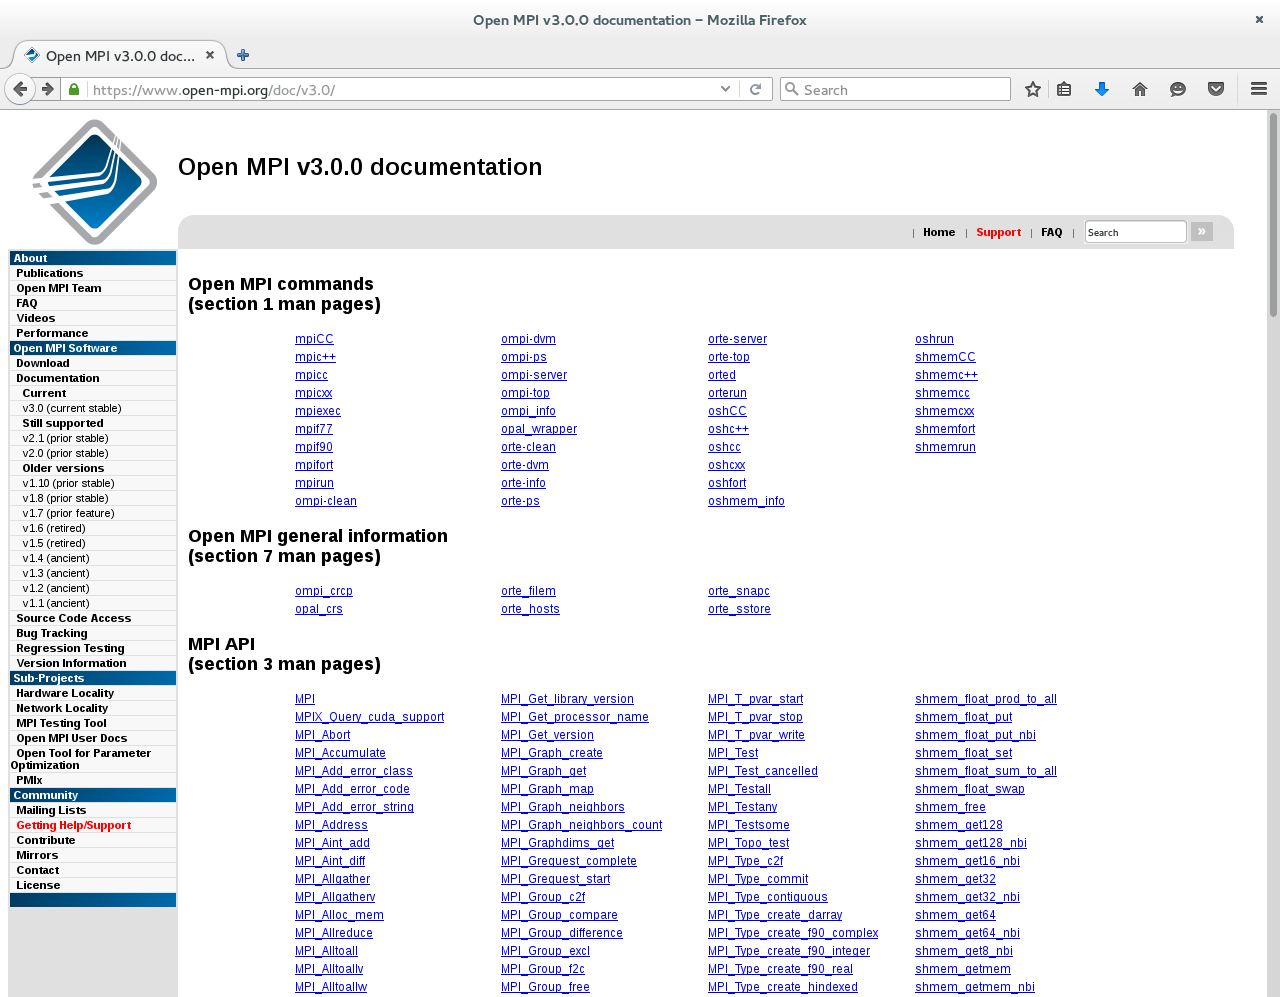
\includegraphics[width=\textwidth]{graphics/openmpi.png}
  \caption{OpenMPI v3.0 documentation page: \url{https://www.open-mpi.org/doc/v3.0/}}
\end{figure}


\Level 0 {MPI collective communication exercises}
\label{sec:collective-mpi-exercises}

Below there are some exercises to familiarize yourself with the collective communication features
of MPI, as seen in section \ref{sec:collective-mpi}.

You can find solutions to these exercises in section
\ref{app:sol-collective-mpi}, but you are \emph{highly encouraged} to try to
solve them first on your own.

\Level 1 {Broadcast}
\label{ex:collective-mpi-broadcast}

This exercise was taken from the "Training MPI" course by CINECA-SCAI. For
details see \url{http://www.hpc.cineca.it/content/exercise-7} 

Task 0 initializes a variable to a given value,then modifies the variable (for
example, by calculating the square of its value) and finally broadcasts it to
all the others tasks.


\Level 1 {Trapezoidal rule integral with I/O}
\label{ex:collective-mpi-trapezoidal-io}

Modify the program for the calculation of an integral using the trapezodial rule
(see \ref{sec:trapezoidal-rule}), so that a,b and n are read by rank 0 and they
are distributed (with collective calls) to the other processes.


\Level 1 {Divide and update array}
\label{ex:collective-mpi-scatter}
This exercise was taken from the "Training MPI" course by CINECA-SCAI. For
details see \url{http://www.hpc.cineca.it/content/exercise-8} 

Task 0 initializes a one-dimensional array assigning to each cell the value of
its index. This array is then divided into chunks and sent to other
processes. After having received the proper chunk, each process updates it by
adding its rank and then sends it back to root process. (Analyze the cases for
equal and not equal chunks separately).

Start by assuming that the length of the array is divisible by the number of
processes. To make it more general, instead of using the routines MPI\_GATHER y
MPI\_SCATTER you should check the documentation for these two routines:
MPI\_GATHERV (https://www.open-mpi.org/doc/v3.0/man3/MPI\_Gatherv.3.php) and
MPI\_SCATTER\_V (https://www.open-mpi.org/doc/v3.0/man3/MPI\_Scatterv.3.php). 



\Level 1 {Reduce operations}
\label{ex:collective-mpi-reduce}
Ejercicio 9 del curso "Training MPI" de CINECA-SCAI. Ver detalles en
\url{http://www.hpc.cineca.it/content/exercise-9}

Each process initializes a one-dimensional array by giving to all the elements
the value of its rank+1. Then the root process (task 0) performs two reduce
operations (sum and then product) to the arrays of all the processes. Finally,
each process generates a random number and root process finds (and prints) the
maximum value among these random values.
 
Modify (optional) the code to perform a simple scalability test using MPI\_Wtime. Notice
what happens when you go up with the number of processes involved.

In Fortran, in order to generate a ``random'' number, you can do:

\begin{verbatim}
REAL :: x
CALL RANDOM_SEED()
CALL RANDOM_NUMBER(x)
\end{verbatim}



\Level 1 {Heat equation - 2D}
\label{ex:collective-mpi-heat2d}
Parallelize the following serial code, which follows the pattern that you would
have to use in order to solve the 2D equation.

\begin{verbatim}

PROGRAM heat2D
  IMPLICIT NONE

  INTEGER :: side, i, j, t=0
  REAL :: min,max,diff
  REAL, DIMENSION( : , : ), ALLOCATABLE :: datu

  READ*, side
  ALLOCATE(datu(0:side+1,0:side+1))

  datu = 0.0
  DO i=1,side
     READ*, datu(i,1:side)
  END DO

  min=MINVAL(datu(1:side,1:side))
  max=MAXVAL(datu(1:side,1:side))
  diff=max-min
  PRINT*, "t = ",t, "diff = ",diff

  DO WHILE (diff .GE. 1)
     t=t+1
     datu(1:side,1:side) = 0.99*datu(1:side,1:side) + 0.01*((datu(0:side-1,1:side) + &
          datu(2:side+1,1:side) + datu(1:side,0:side-1) + datu(1:side,2:side+1)) / 4)
     min=MINVAL(datu(1:side,1:side))
     max=MAXVAL(datu(1:side,1:side))
     diff=max-min
     IF (MOD(t,1000) .EQ. 0) PRINT*, "t = ",t, "diff = ",diff
  END DO
  PRINT*, "Final t is: ", t

END PROGRAM heat2D
\end{verbatim}

This code simply reads an array (let's imagine it represents temperature), which
is updated in each loop. For each of these loops (representing a time step), the
array is updated at each point with this simple expression:

\begin{verbatim}
ti,j = 0.99*ti,j + 0.01*((ti-1,j+ti+1,j+ti,j-1+ti,j+1)/4)
\end{verbatim}

This is computed while the difference between the minimum and maximum values of
the array is $>=$1. We also print this difference for every 1000 time steps, and
at the end we print the total number of time steps given. To verify that your
code is working, you can use the following array (first line gives the array
side, so in this case we are reading a 10x10 array):

\begin{verbatim}

10
1 5 5 5 5 5 5 5 5 5 
5 1 5 5 5 5 5 5 5 5 
5 5 1 5 5 5 5 5 5 5 
5 5 5 1 5 5 5 5 5 5 
5 5 5 5 1 5 5 5 5 5 
5 5 5 5 5 1 5 5 5 5 
5 5 5 5 5 5 1 5 5 5 
5 5 5 5 5 5 5 1 5 5 
5 5 5 5 5 5 5 5 1 5 
5 5 5 5 5 5 5 5 5 1
\end{verbatim}

With this array, the serial program gives:

\begin{verbatim}
angelv$ ./heat2D < temp.in
 t =            0 diff =    4.00000000    
 t =         1000 diff =    3.61902761    
 t =         2000 diff =    2.80383563    
 t =         3000 diff =    1.92610180    
 t =         4000 diff =    1.29235637    
 Final t is:         4636
\end{verbatim}

Your goal is to parallelize this code. Some comments that can help you with this task:

\begin{itemize}
\item To simplify, we can assume that your code will always run in 4 processes
  and that the array side is multiple of 2 (so, when dividing the array in 4
  chunks, each chunk has the same number of elements). But you have to make sure
  that the code works for any array size (as far as the side is multiple of 2).
\item Besides the basic initialization and finalization MPI calls, you can solve
  this problem using only: MPI\_BCAST, MPI\_ALLREDUCE, MPI\_Send and MPI\_Recv
\item Don't try to modify all the code in one go (parallel programs are much
  more difficult to debug than serial ones. Try to change the code in a number
  of steps and making sure that each step gives the correct results:
\begin{itemize}
\item rank 0 just reads the array and distributes it to the other processes
\item now write the part of the program before the loop, where you will
  determine which chunk of the array each process will be responsible for, and
  calculate the initial difference between minimum and maximum values.
\item now go for the loop. The first thing to do (and probably the most
  complicated part of the program) is to determine which information you will
  have to communicate from process to process. Only after you have a clear idea
  of who sends what, then try to write the right MPI routines to perform that communication.
\end{itemize}
\end{itemize}
